\documentclass[letterpaper,10pt, onecolumn]{IEEEtran}

\usepackage{graphicx}                                        
\usepackage{amssymb}                                         
\usepackage{amsmath}                                         
\usepackage{amsthm}                                          

\usepackage{alltt}                                           
\usepackage{float}
\usepackage{color}
\usepackage{fancyvrb}
\usepackage{url}

\usepackage{balance}
\usepackage[TABBOTCAP, tight]{subfigure}
\usepackage{enumitem}
\usepackage{pstricks, pst-node}
\usepackage{minted}

\usepackage{geometry}
\geometry{textheight=8.5in, textwidth=6in}

%random comment

\newcommand{\cred}[1]{{\color{red}#1}}
\newcommand{\cblue}[1]{{\color{blue}#1}}

\newcommand{\toc}{\tableofcontents}

%\usepackage{hyperref}

\def\name{Thomas Albertine}
\title{The Many Faces of Microbial Communities \\\large Senior Design\\Winter Term\\}
\author{\name, Michael Phelps}


%% The following metadata will show up in the PDF properties
% \hypersetup{
%   colorlinks = false,
%   urlcolor = black,
%   pdfauthor = {\name},
%   pdfkeywords = {capstone visualization microbiology microbio senior design},
%   pdftitle = {Senior Design Project, Visualizing Microbial Communities},
%   pdfsubject = {Senior Design Microbiology Visualizations},
%   pdfpagemode = UseNone
% }

\parindent = 0.0 in
\parskip = 0.1 in

\linespread{1.0}

\usepackage{fancyvrb}
\usepackage{color}
\usepackage[latin1]{inputenc}


\makeatletter
\def\PY@reset{\let\PY@it=\relax \let\PY@bf=\relax%
    \let\PY@ul=\relax \let\PY@tc=\relax%
    \let\PY@bc=\relax \let\PY@ff=\relax}
\def\PY@tok#1{\csname PY@tok@#1\endcsname}
\def\PY@toks#1+{\ifx\relax#1\empty\else%
    \PY@tok{#1}\expandafter\PY@toks\fi}
\def\PY@do#1{\PY@bc{\PY@tc{\PY@ul{%
    \PY@it{\PY@bf{\PY@ff{#1}}}}}}}
\def\PY#1#2{\PY@reset\PY@toks#1+\relax+\PY@do{#2}}

\expandafter\def\csname PY@tok@gd\endcsname{\def\PY@tc##1{\textcolor[rgb]{0.63,0.00,0.00}{##1}}}
\expandafter\def\csname PY@tok@gu\endcsname{\let\PY@bf=\textbf\def\PY@tc##1{\textcolor[rgb]{0.50,0.00,0.50}{##1}}}
\expandafter\def\csname PY@tok@gt\endcsname{\def\PY@tc##1{\textcolor[rgb]{0.00,0.25,0.82}{##1}}}
\expandafter\def\csname PY@tok@gs\endcsname{\let\PY@bf=\textbf}
\expandafter\def\csname PY@tok@gr\endcsname{\def\PY@tc##1{\textcolor[rgb]{1.00,0.00,0.00}{##1}}}
\expandafter\def\csname PY@tok@cm\endcsname{\let\PY@it=\textit\def\PY@tc##1{\textcolor[rgb]{0.25,0.50,0.50}{##1}}}
\expandafter\def\csname PY@tok@vg\endcsname{\def\PY@tc##1{\textcolor[rgb]{0.10,0.09,0.49}{##1}}}
\expandafter\def\csname PY@tok@m\endcsname{\def\PY@tc##1{\textcolor[rgb]{0.40,0.40,0.40}{##1}}}
\expandafter\def\csname PY@tok@mh\endcsname{\def\PY@tc##1{\textcolor[rgb]{0.40,0.40,0.40}{##1}}}
\expandafter\def\csname PY@tok@go\endcsname{\def\PY@tc##1{\textcolor[rgb]{0.50,0.50,0.50}{##1}}}
\expandafter\def\csname PY@tok@ge\endcsname{\let\PY@it=\textit}
\expandafter\def\csname PY@tok@vc\endcsname{\def\PY@tc##1{\textcolor[rgb]{0.10,0.09,0.49}{##1}}}
\expandafter\def\csname PY@tok@il\endcsname{\def\PY@tc##1{\textcolor[rgb]{0.40,0.40,0.40}{##1}}}
\expandafter\def\csname PY@tok@cs\endcsname{\let\PY@it=\textit\def\PY@tc##1{\textcolor[rgb]{0.25,0.50,0.50}{##1}}}
\expandafter\def\csname PY@tok@cp\endcsname{\def\PY@tc##1{\textcolor[rgb]{0.74,0.48,0.00}{##1}}}
\expandafter\def\csname PY@tok@gi\endcsname{\def\PY@tc##1{\textcolor[rgb]{0.00,0.63,0.00}{##1}}}
\expandafter\def\csname PY@tok@gh\endcsname{\let\PY@bf=\textbf\def\PY@tc##1{\textcolor[rgb]{0.00,0.00,0.50}{##1}}}
\expandafter\def\csname PY@tok@ni\endcsname{\let\PY@bf=\textbf\def\PY@tc##1{\textcolor[rgb]{0.60,0.60,0.60}{##1}}}
\expandafter\def\csname PY@tok@nl\endcsname{\def\PY@tc##1{\textcolor[rgb]{0.63,0.63,0.00}{##1}}}
\expandafter\def\csname PY@tok@nn\endcsname{\let\PY@bf=\textbf\def\PY@tc##1{\textcolor[rgb]{0.00,0.00,1.00}{##1}}}
\expandafter\def\csname PY@tok@no\endcsname{\def\PY@tc##1{\textcolor[rgb]{0.53,0.00,0.00}{##1}}}
\expandafter\def\csname PY@tok@na\endcsname{\def\PY@tc##1{\textcolor[rgb]{0.49,0.56,0.16}{##1}}}
\expandafter\def\csname PY@tok@nb\endcsname{\def\PY@tc##1{\textcolor[rgb]{0.00,0.50,0.00}{##1}}}
\expandafter\def\csname PY@tok@nc\endcsname{\let\PY@bf=\textbf\def\PY@tc##1{\textcolor[rgb]{0.00,0.00,1.00}{##1}}}
\expandafter\def\csname PY@tok@nd\endcsname{\def\PY@tc##1{\textcolor[rgb]{0.67,0.13,1.00}{##1}}}
\expandafter\def\csname PY@tok@ne\endcsname{\let\PY@bf=\textbf\def\PY@tc##1{\textcolor[rgb]{0.82,0.25,0.23}{##1}}}
\expandafter\def\csname PY@tok@nf\endcsname{\def\PY@tc##1{\textcolor[rgb]{0.00,0.00,1.00}{##1}}}
\expandafter\def\csname PY@tok@si\endcsname{\let\PY@bf=\textbf\def\PY@tc##1{\textcolor[rgb]{0.73,0.40,0.53}{##1}}}
\expandafter\def\csname PY@tok@s2\endcsname{\def\PY@tc##1{\textcolor[rgb]{0.73,0.13,0.13}{##1}}}
\expandafter\def\csname PY@tok@vi\endcsname{\def\PY@tc##1{\textcolor[rgb]{0.10,0.09,0.49}{##1}}}
\expandafter\def\csname PY@tok@nt\endcsname{\let\PY@bf=\textbf\def\PY@tc##1{\textcolor[rgb]{0.00,0.50,0.00}{##1}}}
\expandafter\def\csname PY@tok@nv\endcsname{\def\PY@tc##1{\textcolor[rgb]{0.10,0.09,0.49}{##1}}}
\expandafter\def\csname PY@tok@s1\endcsname{\def\PY@tc##1{\textcolor[rgb]{0.73,0.13,0.13}{##1}}}
\expandafter\def\csname PY@tok@sh\endcsname{\def\PY@tc##1{\textcolor[rgb]{0.73,0.13,0.13}{##1}}}
\expandafter\def\csname PY@tok@sc\endcsname{\def\PY@tc##1{\textcolor[rgb]{0.73,0.13,0.13}{##1}}}
\expandafter\def\csname PY@tok@sx\endcsname{\def\PY@tc##1{\textcolor[rgb]{0.00,0.50,0.00}{##1}}}
\expandafter\def\csname PY@tok@bp\endcsname{\def\PY@tc##1{\textcolor[rgb]{0.00,0.50,0.00}{##1}}}
\expandafter\def\csname PY@tok@c1\endcsname{\let\PY@it=\textit\def\PY@tc##1{\textcolor[rgb]{0.25,0.50,0.50}{##1}}}
\expandafter\def\csname PY@tok@kc\endcsname{\let\PY@bf=\textbf\def\PY@tc##1{\textcolor[rgb]{0.00,0.50,0.00}{##1}}}
\expandafter\def\csname PY@tok@c\endcsname{\let\PY@it=\textit\def\PY@tc##1{\textcolor[rgb]{0.25,0.50,0.50}{##1}}}
\expandafter\def\csname PY@tok@mf\endcsname{\def\PY@tc##1{\textcolor[rgb]{0.40,0.40,0.40}{##1}}}
\expandafter\def\csname PY@tok@err\endcsname{\def\PY@bc##1{\setlength{\fboxsep}{0pt}\fcolorbox[rgb]{1.00,0.00,0.00}{1,1,1}{\strut ##1}}}
\expandafter\def\csname PY@tok@kd\endcsname{\let\PY@bf=\textbf\def\PY@tc##1{\textcolor[rgb]{0.00,0.50,0.00}{##1}}}
\expandafter\def\csname PY@tok@ss\endcsname{\def\PY@tc##1{\textcolor[rgb]{0.10,0.09,0.49}{##1}}}
\expandafter\def\csname PY@tok@sr\endcsname{\def\PY@tc##1{\textcolor[rgb]{0.73,0.40,0.53}{##1}}}
\expandafter\def\csname PY@tok@mo\endcsname{\def\PY@tc##1{\textcolor[rgb]{0.40,0.40,0.40}{##1}}}
\expandafter\def\csname PY@tok@kn\endcsname{\let\PY@bf=\textbf\def\PY@tc##1{\textcolor[rgb]{0.00,0.50,0.00}{##1}}}
\expandafter\def\csname PY@tok@mi\endcsname{\def\PY@tc##1{\textcolor[rgb]{0.40,0.40,0.40}{##1}}}
\expandafter\def\csname PY@tok@gp\endcsname{\let\PY@bf=\textbf\def\PY@tc##1{\textcolor[rgb]{0.00,0.00,0.50}{##1}}}
\expandafter\def\csname PY@tok@o\endcsname{\def\PY@tc##1{\textcolor[rgb]{0.40,0.40,0.40}{##1}}}
\expandafter\def\csname PY@tok@kr\endcsname{\let\PY@bf=\textbf\def\PY@tc##1{\textcolor[rgb]{0.00,0.50,0.00}{##1}}}
\expandafter\def\csname PY@tok@s\endcsname{\def\PY@tc##1{\textcolor[rgb]{0.73,0.13,0.13}{##1}}}
\expandafter\def\csname PY@tok@kp\endcsname{\def\PY@tc##1{\textcolor[rgb]{0.00,0.50,0.00}{##1}}}
\expandafter\def\csname PY@tok@w\endcsname{\def\PY@tc##1{\textcolor[rgb]{0.73,0.73,0.73}{##1}}}
\expandafter\def\csname PY@tok@kt\endcsname{\def\PY@tc##1{\textcolor[rgb]{0.69,0.00,0.25}{##1}}}
\expandafter\def\csname PY@tok@ow\endcsname{\let\PY@bf=\textbf\def\PY@tc##1{\textcolor[rgb]{0.67,0.13,1.00}{##1}}}
\expandafter\def\csname PY@tok@sb\endcsname{\def\PY@tc##1{\textcolor[rgb]{0.73,0.13,0.13}{##1}}}
\expandafter\def\csname PY@tok@k\endcsname{\let\PY@bf=\textbf\def\PY@tc##1{\textcolor[rgb]{0.00,0.50,0.00}{##1}}}
\expandafter\def\csname PY@tok@se\endcsname{\let\PY@bf=\textbf\def\PY@tc##1{\textcolor[rgb]{0.73,0.40,0.13}{##1}}}
\expandafter\def\csname PY@tok@sd\endcsname{\let\PY@it=\textit\def\PY@tc##1{\textcolor[rgb]{0.73,0.13,0.13}{##1}}}

\def\PYZbs{\char`\\}
\def\PYZus{\char`\_}
\def\PYZob{\char`\{}
\def\PYZcb{\char`\}}
\def\PYZca{\char`\^}
\def\PYZam{\char`\&}
\def\PYZlt{\char`\<}
\def\PYZgt{\char`\>}
\def\PYZsh{\char`\#}
\def\PYZpc{\char`\%}
\def\PYZdl{\char`\$}
\def\PYZti{\char`\~}
% for compatibility with earlier versions
\def\PYZat{@}
\def\PYZlb{[}
\def\PYZrb{]}
\makeatother


\begin{document}
\maketitle
\section*{Abstract}
We intend for this project to provide a better way to visualize microbial population data than some existing techniques. We currently have working backend components for loading population data files, generating models, and converting population counts into normalized values that can be used to generate models, as well as a preliminary UI for most of our project. However, we still need to finish the rest of our UI and add backend functionality for grouping. Once we've worked out the most obvious flaws in our project, we will perform a small number of moderated, in-person tests, that should point out additional flaws which we may have overlooked. 

Of the code that we've written thus far, the most difficult challenge we've faced was simply to dig through the MakeHuman source code in order to write a wrapper. 

Thomas Albertine has written the majority of this document because he has a cold, and therefore would like to avoid being in the video presentation as much as possible.

\clearpage
\section*{Purposes and Goals}

The purpose of the project is to visualize microbial population data in a way that allows microbiologists (and secondarily other researchers) to better compare complex population data. To that effect, our client has requested that we model it as human-esque faces, in order to take advantage of humans' ability to recognize and compare those faces. Resulting models need not look like visually appealing humans, but they should represent the data.

\section*{Completed Content}

\subsection*{Backend}

\begin{figure}
	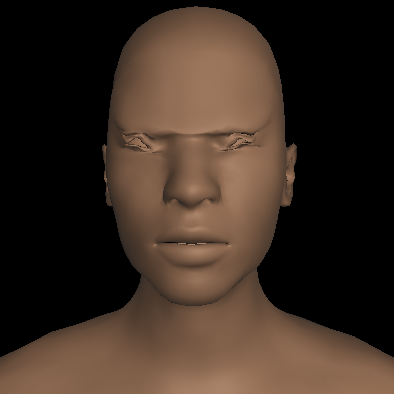
\includegraphics{Generated}
	\caption{A model generated from a sample data file. This file had few enough organisms that only some features were modified. The rest were left at their default values to avoid distracting from the significant features. The model viewer this was taken with is the built-in Windows 10 model viewer.}
	\label{fig:generated}
\end{figure}

In the backend code of the project, Thomas has already written a wrapper around makehuman that can retrieve valid model parameter names\footnote{Our requirements document specifies that we support 150 model parameters, but we only have enough facial features to support 138. We can extend that number significantly however, if we use other model parameters besides facial features, but our client mainly wants to work with facial features alone. We are considering adding the others as optional parameters.} as well as receive model parameter names and values in order to generate models. This particular code has a minor deficiency in that the models it produces have no eyes, so if we have time to improve upon it later, we intend to. That said, if it proves impossible, the current system is still sufficient to visualize the data. Figure \ref{fig:generated} depicts a model generated from a data file. The code can be found in $modelGenerator.py$.

Thomas\footnote{Originally, Michael started writing this component, but there was a miscommunication and Thomas panicked and wrote it instead.} has also written code to load an QIIME OTU tab-delineated data file, as well as framework to allow us to easily add support for other file types later on. This is described in more detail in the ``Interesting Code'' section later in this document, but in short, we've created parser objects which we associate with file extensions in a registry object which we have created. When loading a file, simply pass the file path into the registry object, and it uses the extension from the path to find the right parser, which is passed the file path. This code can be found in $otuParser.py$ and $fvParser.py$.

Thomas has also written code to normalize sample data based on the largest population in the sample (to compare ratios of populations between samples), based on the largest population in the file (to compare population sizes between samples), and a manual scaling value that can be set by the user, in order to compare between images of previously generated models, or models in separate files. This code can be found in $modelGeneratorTranslator.py$.

Finally we have a test script that demonstrates the functionality of the backend components. It resides in $test.py$.

\subsection*{Frontend}

Michael has written the data loading page as well as the main selection page, and he is currently working on the detailed viewing page. Currently, none of the UI elements actually do anything, but we will be ready to start linking the UI with the backend functionality soon.

\begin{figure}
	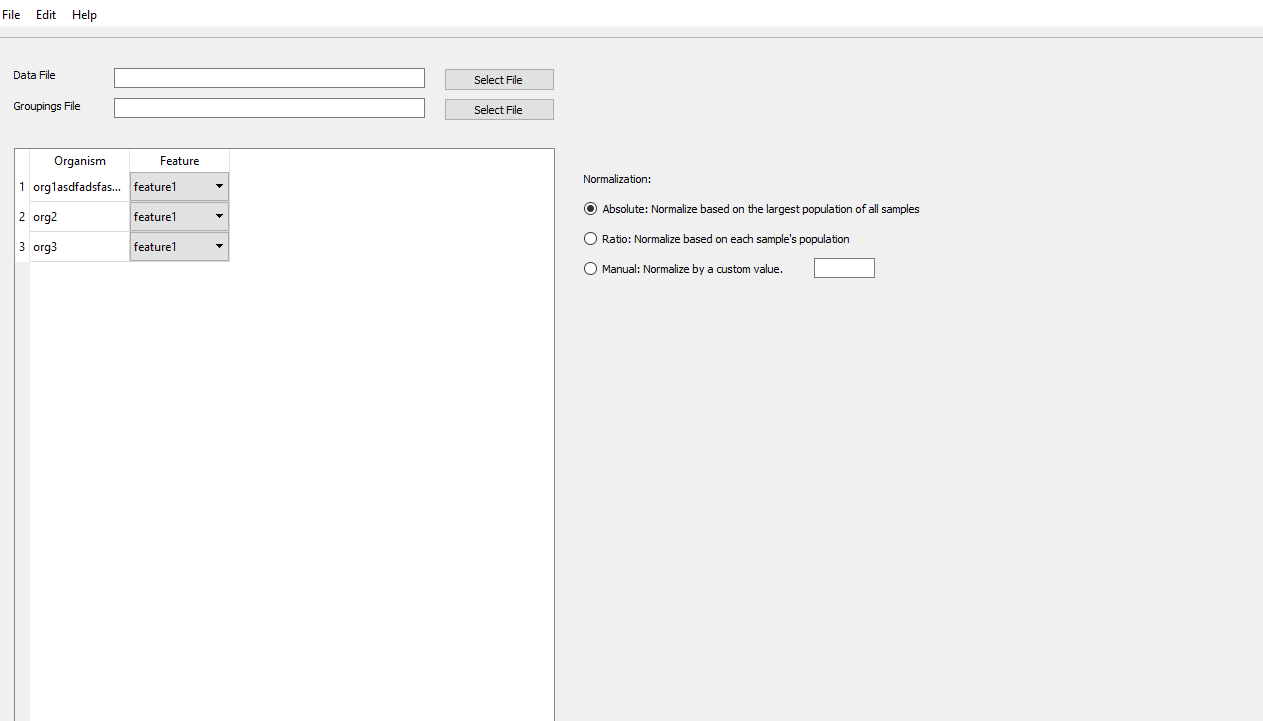
\includegraphics[width=\textwidth]{LoadingInterface}
	\caption{The UI page that allows users to perform taks related to loading data files.}
	\label{fig:LoadingInterface}
\end{figure}

The Data Loading page (see Figure \ref{fig:LoadingInterface}) will allow users to select a data file and a groupings file. These files will be loaded, and then used to populate the table on the left, which allows users to associate model parameters with organisms in the sample. On the right, a series of radio buttons can be used to specify which normalizing strategy to use.

\begin{figure}
	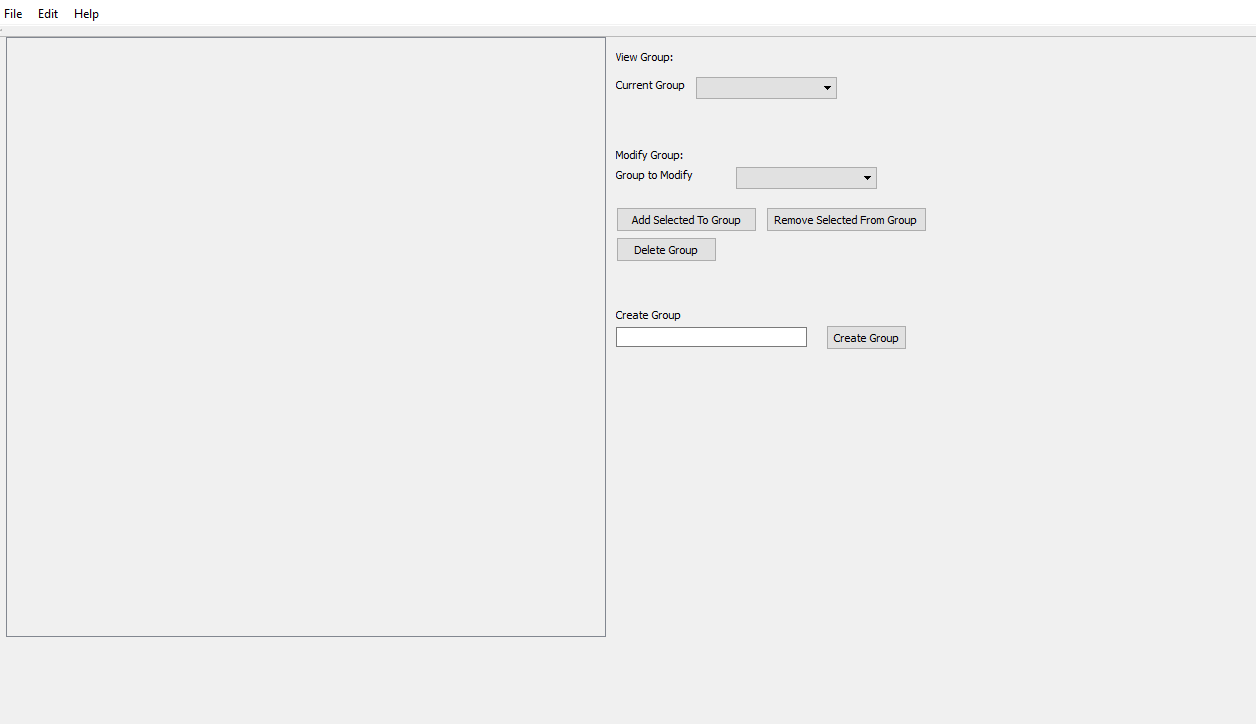
\includegraphics[width=\textwidth]{MainInterface}
	\caption{The UI page that allows users to perform taks related to selecting data files.}
	\label{fig:MainInterface}
\end{figure}

The Main Selection page (see Figure \ref{fig:MainInterface}) will allow users to select a few samples out of the file to examine in more detail. The box on the left is where images of the samples' models will appear, while the elements on the right are for the grouping functionality.

\section*{Remaining Content}

As mentioned in the previous section, the UI is not finished, and does not yet interact at all with the backend. The pages that do exist need to be polished as well. The Loading page needs a button for the user to indicate that he or she is finished on the page. The Main Selection Page needs a button to indicate that the user has selected the models to analyze. Both are larger than is convenient on a smaller screen, and the layouts are absolute, so scaling the window moves elements outside the viewing area. We also don't yet have a way to draw the models, but we believe that this can be done within PyQT, and we are currently working on it.

As mentioned in the backend section, if time allows, we would also fix the eye problem with model generation and improve our testing.

There is currently little work done with grouping. The parser will eventually be able to load groups along with data files, since groups can be passed in as metadata files in the QIIME OTU standard. Additionally, those groups will be modifiable and viewable later on the Selection page.

\section*{Significant Problems and Associated Solutions}

The most difficult problem that Thomas faced was simply trying to read and decypher the MakeHuman code enough to write the wrapper. Since Python is loosely typed, he couldn't just match the types to see how things were being used. Instead (at least at first), he had to walk through the code jumping from function definition to function definition, searching through multiple files. After doing that for a few hours, he remembered that python objects have a dictionary of their attributes, so he was able to import MakeHuman modules and examine the the contents of objects returned from functions. This sped up the process considerably. Additionally, he figured out how to use grep-like functionality from within PowerShell, which made it much easier to look for function definitions.

Here, Michael will describe his most difficult problem thus far.

\section*{Interesting Code}

The Following is the framework for easy addition of new parsers. minParser represents the minimum functionality required for a parser. If this were C++, it would be a virtual class, but thanks to Python's duck typing, we don't actually have to inherit from anything, so it's more of a template for us to copy later.

The ParserRegistry itself is little more than a wrapper around a dictionary, mapping a file extension to a parser object, but with some additional functions added to it to make its usage more obvious. Finally, an instance of the Registry is created as a global, so that it can be referenced anywhere by importing the module.

\inputminted{python}{../../code/FaceView/fvParser.py}

\section*{User Study}

As of now, the only feedback we have regarding usability is from our client, about our mockup. She happens to be a member of our target audience, so this is a good sign, but it isn't enough validation. We need to do a user study once we fix some of the more obvious problems, and connect it to the backend functionality.

\subsection*{Users}

Our target users are microbiology researchers, but we don't have access to many of them. However, if users with no prior knowledge of our application and rudimentary computer skills can learn to use our application quickly, then surely researchers should have no trouble. In any case, there's certainly more generic users than there are microbiology researchers.

\subsection*{Methods}

We plan to use a set of 5 moderated, in-person tests at this stage. This should be enough to identify some stumbling blocks, but not so many that it takes an impractical amount of time to moderate it.

\subsection*{Tasks}

Before each task, we will ask users how confident they are that they can complete the task, and we will time them while they are performing the task, recording the time it takes them. If we see them struggling over a particular step in the task, we will make a note of it. If the user exceeds the specified time limit for the task, we will make a note of what step they were stuck on, politely interrupt them, and complete the step ourselves if the next task requires it. If they request that we repeat the question, we will oblige. If they request clarification, we will make a note of that as well, so that we can design a better test in the future.

Our tasks are as follows, starting immediately after opening the application for the first time, and given a sample data file:
\begin{enumerate}
	\item Load the data file. (30 seconds)
	\item Associate Bacillus subtilis with head squareness\footnote{This organism and this model parameter need not be the ones used in the test}. (30 seconds)
	\item Modify settings so that you can compare ratios of different populations between samples. (20 seconds)
	\item Generate the models. (20 seconds)
	\item Select some samples to compare in more detail. (30 seconds)
	\item Manipulate the models. (20 seconds)
	\item Navigate to the screen where you selected samples to compare in more detail. (30 seconds)
	\item Find the two samples with the most similar ratios of Bacillus subtilis to total population and view them in more detail. (3 minutes)
	\item Find the two samples with the most similar total population of bacillus subtilis and view them in more detail. (3 minutes)
\end{enumerate}

The first seven tasks are primarily to identify how intuitive the application is to a new user. The last two are to identify how easy the application is to use once someone has seen how it works.

\end{document}
